\documentclass[11pt,a4paper]{article}

\usepackage{latexsym}
\usepackage[left=1.5cm,right=1.5cm,bottom=2.5cm,top=2.5cm]{geometry}
\usepackage{tikz} 
\usepackage{mathtools} %Math function
\usepackage{listings} %Source code
\usepackage{pdfpages} %PDF import

\pdfinfo{
	/Title (Andrix-Industry.pdf)
	/Creator (Kevin Pan)
	/Producer (PRIA Austria)
	/Author (Kevin Pan)
	/Subject (Andrix Industry - Sample Usage)
	/Keywords (Andrix, Industry, Sample)
}

\usepackage{graphicx}
\lstset{ 
numbers=left
}

\begin{document}


%----------------------------------------------------------------------------------------
%	TITLE PAGE
%----------------------------------------------------------------------------------------

\begin{titlepage}

\newcommand*{\titlePAGE}{\begingroup % Create the command for including the title page in the document
\hbox{ % Horizontal box
\hspace*{0.1\textwidth} % Whitespace to the left of the title page
\rule{1pt}{\textheight} % Vertical line
\hspace*{0.05\textwidth} % Whitespace between the vertical line and title page text
\parbox[b]{0.75\textwidth}{ % Paragraph box which restricts text to less than the width of the page

{\noindent\Huge\bfseries \textit{Andrix Industry} \\ Sample Usage}\\[2\baselineskip] % Title
{\large \textit{Practical Robotic Institude Austria}}\\
{\large \textit{TGM - The Institute of Technology Austria}}\\[1\baselineskip]
{\large \textbf{2015 May}}\\[4\baselineskip]
{\Large \textsc{Kevin Pan}}\\[1\baselineskip]% Author name
{\Large \textsc{Alexander Wurm}} % Author name

\vspace{0.5\textheight} % Whitespace between the title block and the publisher
{\noindent 
\includegraphics[scale=0.25]{img/pria_logo.png} 
\includegraphics[scale=0.6]{img/Tgm_logo.jpg}}\\[\baselineskip] % Publisher and logo
}}
\endgroup}

\titlePAGE % This command includes the title page

\end{titlepage}

%----------------------------------------------------------------------------------------
%	CONTENT TABLE
%----------------------------------------------------------------------------------------

\newpage

\tableofcontents


%----------------------------------------------------------------------------------------
%	GENERAL
%----------------------------------------------------------------------------------------

\newpage
\part{Introduction}

	%###################################################
	%	ABOUT
	%###################################################

\section{About}
\subsection{PRIA}
The Practical Robotics Institute Austria (PRIA) is a non-profit organisation with the aim to promote scientific and technical excellence in schools using robotics as well as the participation and operation of exemplary research projects in fields related to robotics and automation and teaching methods by means of robotics. The Practical Robotics Institute Austria is constituted as an independent non-profit organisation with a scientific advisory board.\\

Robots are sophisticated, intelligent systems used in factories and everyday life. They allow students to connect theory with practice and exercise team work, project management, problem solving and communication skills in a stimulating setting. Robotics integrates all the skills needed for designing and constructing machines, computers, software, communications systems and networks. It conveys to students the flexibility needed for developing interdisciplinary projects and discovers exciting topics such as movement, navigation, coordination, physical interaction with objects, audio and video processing, cognition and recognition and many others. It also helps them in developing their abstract thinking and to acquire teamwork skills, independence, imagination and creativity. Experiments with robots include many hands-on experiments that make classes more dynamic and fun.\\


\subsection{Our Mission}

\begin{itemize}
  \item To use robotics technology as an instrument to prepare students to work with various mechanical, electrical and software systems.
  \item To develop environments and tools for teaching robotics that
    \begin{itemize}
    \item will enable simpler programing and control of robots,
    \item are easily interfaced with a broad range of sensors and effectors,
    \item can be used to investigate complex problems and tasks,
    \item are affordable and open for public use.
  \end{itemize}
  \item To introduce appropriate educational methodologies for the successful integration of robotics innovation in school classes.
  \item To organise robotics competitions and measure their educational impact.
  \item Create innovative control architectures for robotics and industrial automation.
  \item Develop knowledge-based systems and agent technology for the automation of flexible industrial processes.
  \item Introduce Augmented Reality and make visualization of industrial processes more efficient and easier to understand.
\end{itemize}


	%###################################################
	%	Concept
	%###################################################
\newpage
\section{Concept}
\subsection{Idea}
Nowadays computers with ARM architecture are becomming more common. Various smartphones, as well as sigle-board computers like Raspberry Pi are becomming cheaper and much more affordable. To be able to use ARM Devices as robot controllers, some additional hardware that enables connecting and controlling robot components such as sensors, motors and servos are required. The hardware (aka. Low-Level Control, LLC) and the ARM devices(aka. High-Level Control, HLC) should be able to be connected together using both wired and wireless communications.\\

\begin{figure}[htp]
	\centering
	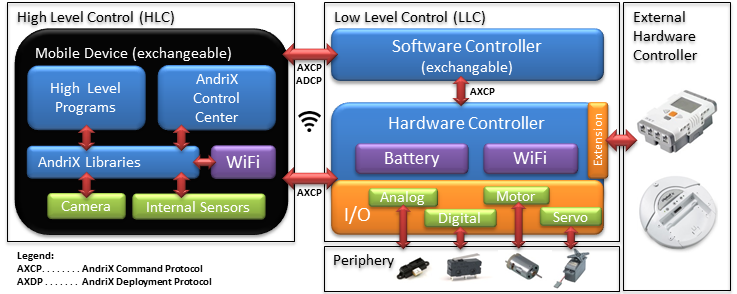
\includegraphics[scale=0.7]{img/Andrix_concept_v3.png}
	\caption{Andrix Concept}
	\label{fig:Andrix Concept v3}
\end{figure}

Andrix Industry is the concept of implementing this kind of structure in an industrial environment and its controller has to be relatively low-cost, stable and expandable for different uses.\\

In this project, we use a standard industrial conveyor belt to test our idea. We will connect  our Andrix controller (including an Raspberry Pi as the High level control) to an external Motor Controller (aka. External Hardware Controller level) to be able to drive the conveyor belt using a Stepper Motor.\\

\begin{figure}[htp]
	\centering
	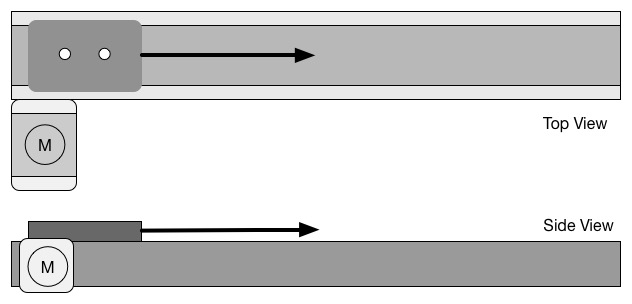
\includegraphics[scale=0.5]{img/Axis_plan.jpg}
	\caption{conveyor belt with NEMA stepper motor}
	\label{fig:Axis Plan}
\end{figure}


THe NEMA Stepper motor series is one of the most popular motors in both amateur and professional fields. They are amazingly  accurate and powerful, but at the same time very easy to control.

	%###################################################
	%	Process
	%###################################################

\newpage
\section{Process}
\subsection{Project steps}
To be able to achive this goal, we planned the project precisely. The following provides a brief overview of our processes:

\begin{enumerate}
\item Choosing matching hardware 
\item Designing necessary mechanical parts
\item Producing mechanical parts by using CNC or 3D-printer 
\item Calculating needed supply power 
\item Designing external motor controller 
\item Prototyping electronic design
\item Communication protocol 
\item Software programming 
\item Debug, test and other final process 
\end{enumerate}

There are some different conditions which have to be satisfied to achieve our concept. At first, we need to find an industrial conveyor belt, which has to be samll enough to let us drive it easily with a stepper-motor without having too many problems. There are mainly two kinds of conveyor belt on the market today - limited and unlimited countineus conveying systems.\\

\subsection{Selecting a suitable conveyor belt}
Unlimited countineus conveying systems are the most common version and have been applied in various areas like raw meterial supply or warehouse transportation systems. They don't need any sesors to detects current position and can be controlled easily by changing the speed of the rotations. Limited conveyor belts work in principle familiar to continues system, but the position of the belt is controlled precisely use servo motor and has integrated sensors working with Hall effect(magnet) or IR encoders(light), but both of them need an extra circuit to drive them and need an externel programme to decode the position.\\

\subsection{Selecting actuator}
This is also one of the reasons why we use a stepper motor. NEMA stepper motors are in comparision to other motors much more flexible. It can be controlled easily with two H-Bridge Motor controller or FET-Transistors. We can dettect the position just by counting the steps in the register from the microcontroller. Of course it also has a disadvantage - speed. The accurency and the speed of the motor are proportional to each other and in our case, this can lead to inaccuracies by changing the step resolution, which is not a mechanical problem that can be easily avoided.\\

\subsection{Communication}
An agreement for the communication protocol between the Andrix and the external motor controller has to be made too. We are using 9600 bit/s as our communication speed. It is a standard bandwidth and can be controlled by other computers. The electronic controller has to be choosed carefully. We have to calculate and test the maximum supply current the motor need to run stably and compare it with the datasheet from the manufactuer.\\

\begin{figure}[htp]
	\centering
	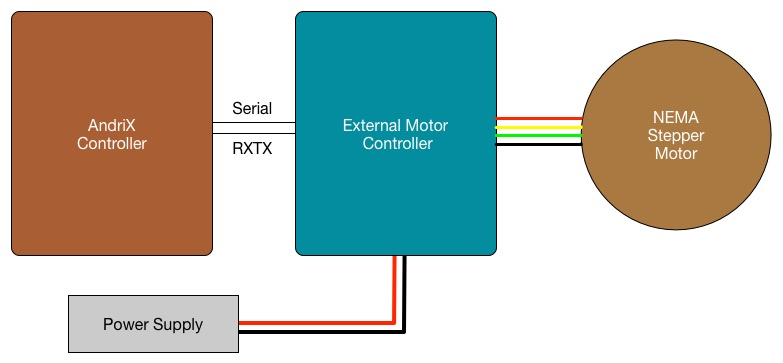
\includegraphics[scale=0.4]{img/Connection_Plan.jpg}
	\caption{Control Flow}
	\label{fig:Axis Plan}
\end{figure}


%----------------------------------------------------------------------------------------
%	DESIGN
%----------------------------------------------------------------------------------------

\newpage
\part{Design}

	%###################################################
	%	Mechanic
	%###################################################
\section{Mechanics}

\subsection{conveyor belt and Axis}

For the conveyor belt, we chose the Bosch RExroth CKR linear motion series. The CKR Compact Modules are precision, ready-to-install linear systems offering high performance within a compact envelope and selectable length, combined with an economical price-to-performance ratio.\\


\textbf{Construction:}
\begin{itemize}
	\item Extremely compact precision aluminum profile with two integrated ball rail guides for optimal movement of heavy loads at high speeds
	\item Ready-to-install Compact Modules in selectable lengths up to Lmax
	\item Short or long aluminum carriage lengths available, depending on application load
	\item Driven by a pre-tensioned, steel-cord reinforced polyurethane toothed belt\\
\end{itemize}

\textbf{Optional Components:}
\begin{itemize}
	\item Maintenance free digital servo drives with integrated brake and pre-installed feedback
	\item Gear Reduced type LP
	\item REED or HALL sensor switches available
	\item Socket with terminals for connection switches
	\item Aluminum profile cable duct for easy mounting of switches\\
\end{itemize}


\textbf{Capabilities:}
\begin{itemize}
	\item Speed - up to 5 m/s
	\item Load Capacity C - up to 56,530 N
	\item Length - up to 5,500mm
	\item Height - 40mm to 65mm
	\item Static Loading - up to 200kg
\end{itemize}

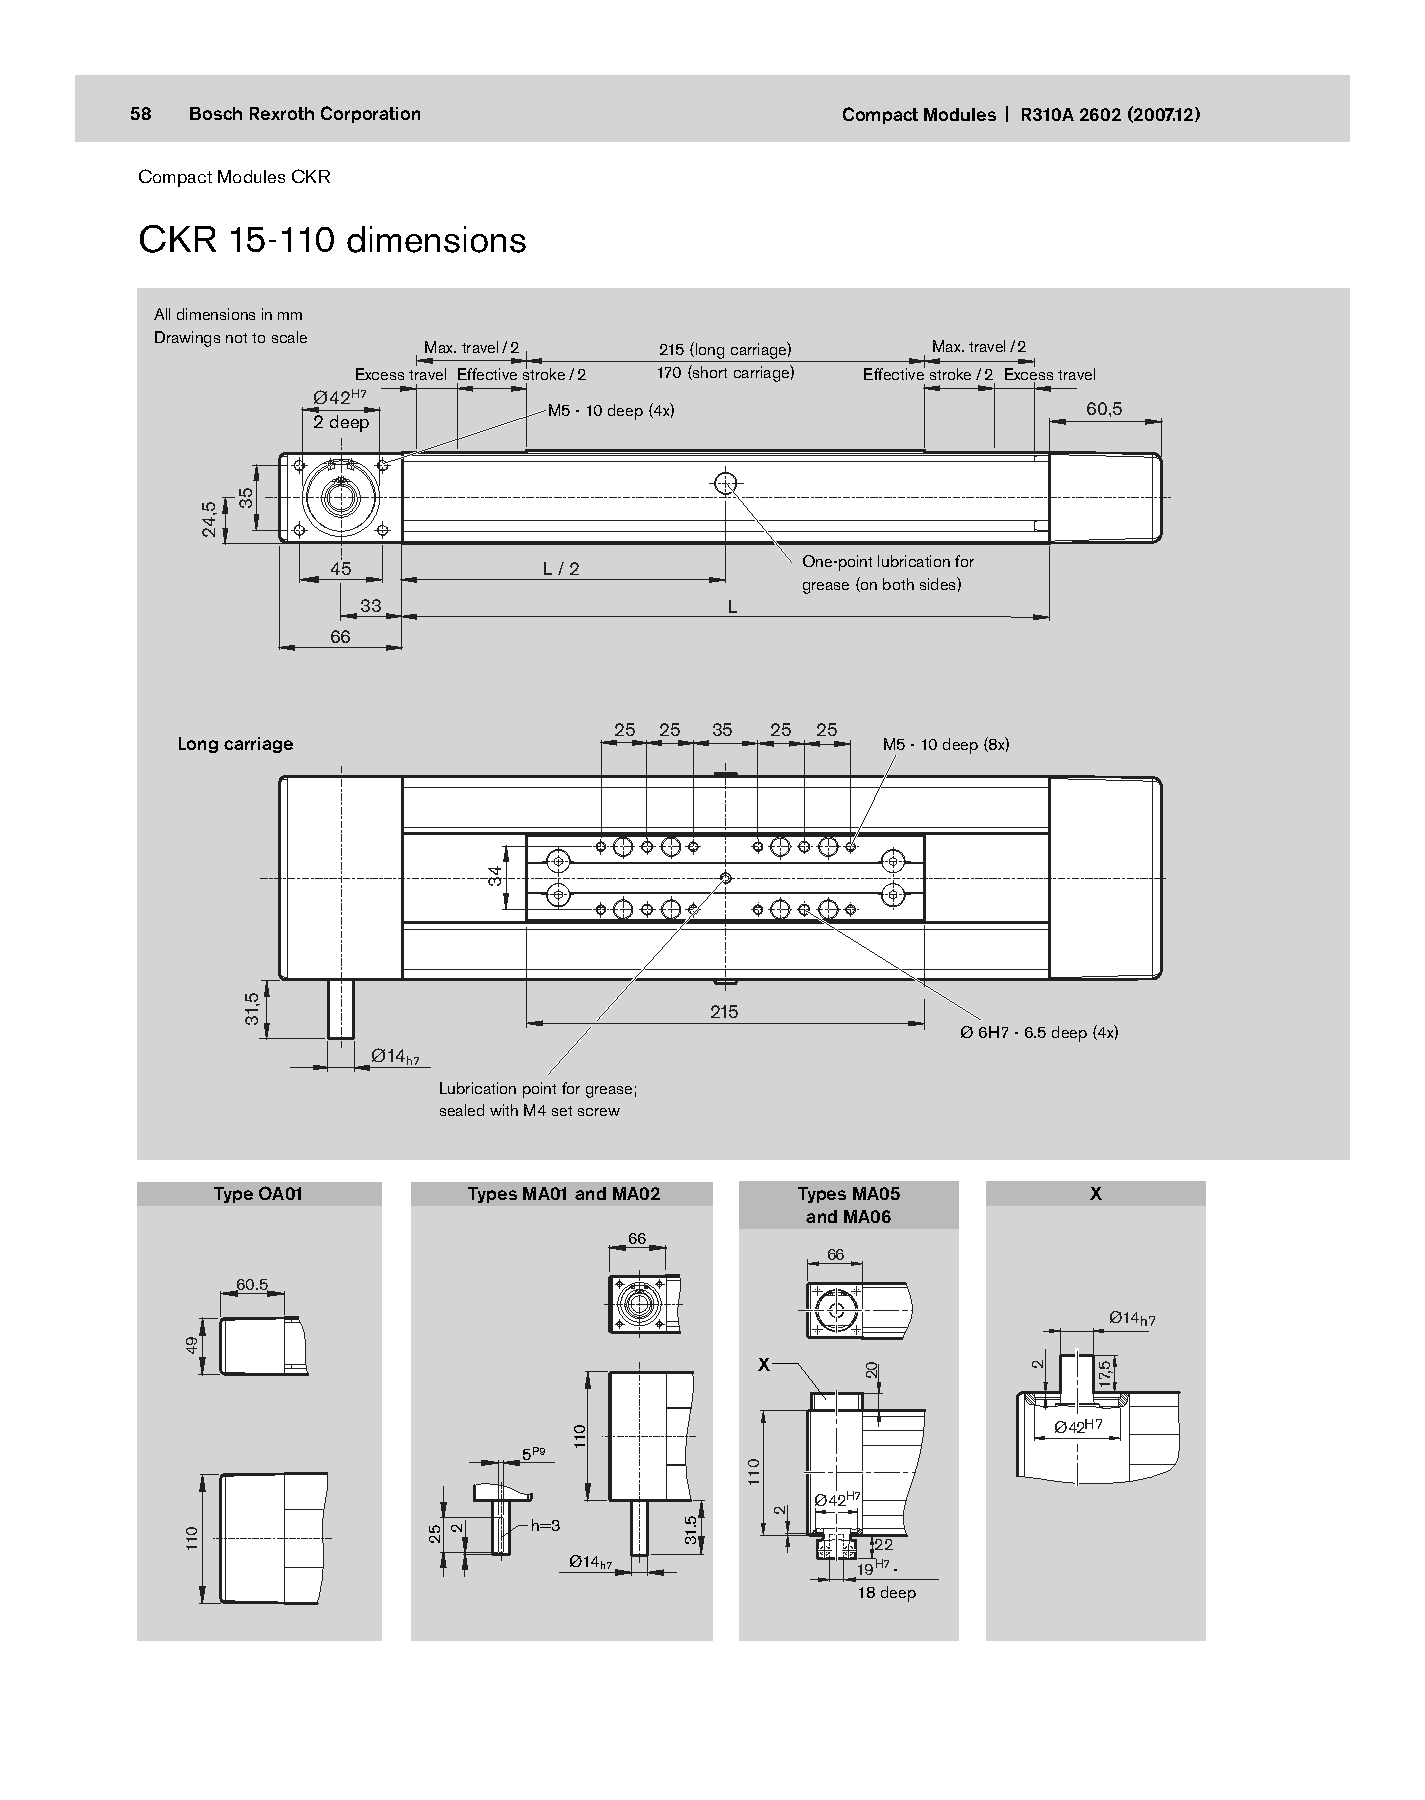
\includepdf[pages=-]{cad/CKR_110_NN_1_69.PDF}
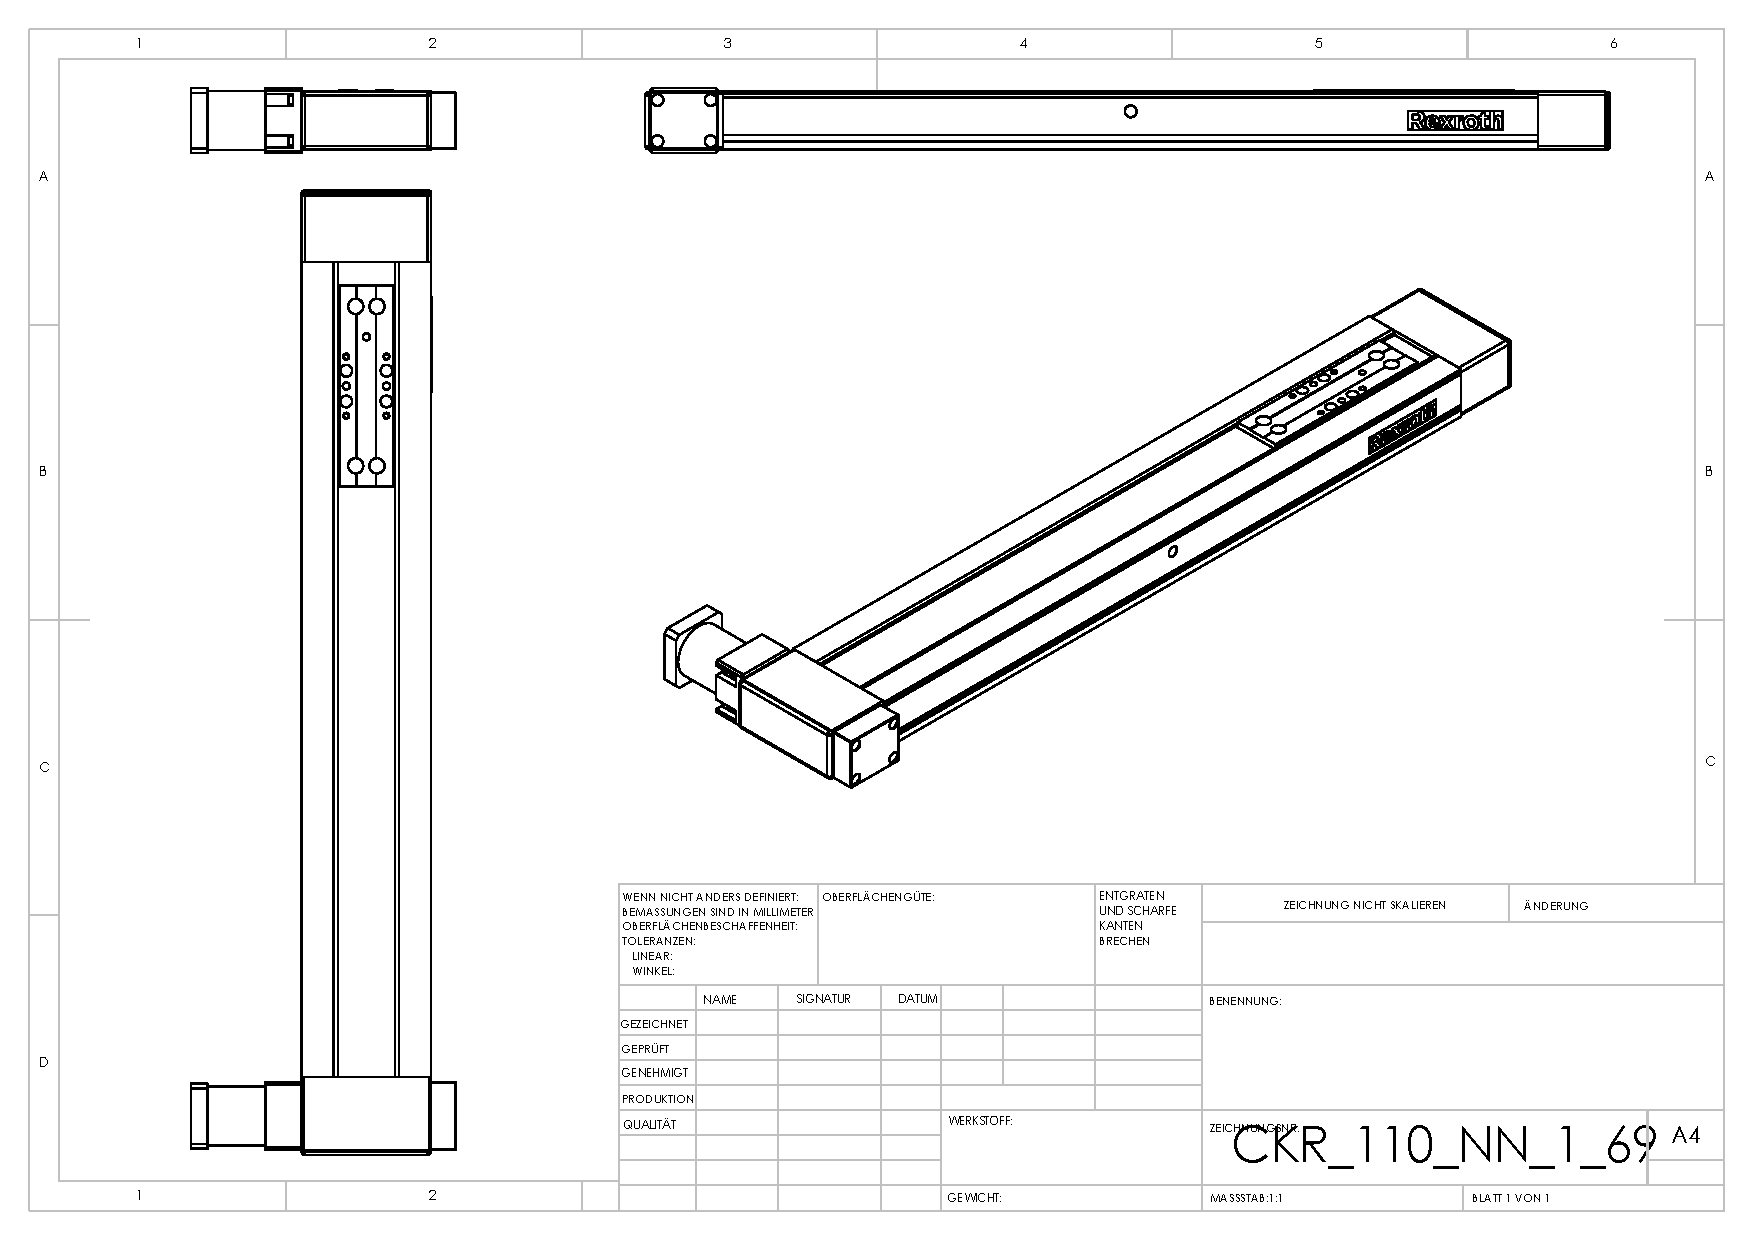
\includepdf[pages=-,landscape]{cad/CKR_110.PDF}

\newpage
\subsection{Actuator and motor}
The motor we are using is QSH5718-76-28-189 from TRINAMIC. It is a two phase hybird stepper motors optimized for microstepping and gives a good fit to high accurate control.\\

\textbf{Specification:}
\begin{itemize}
	\item NEMA 23 mounting Configuration
	\item Number of Leads:	4
	\item Step angle:	1.8
	\item Step Angle Accuracy:	0.05
	\item Holding Torque:	1.89 Nm
	\item Max app. Voltage: 75V
	\item Max Current:	2.8A /Phase	
	\item Max Temp. Rise:	+80
	\item Weight:	1kG
	\item Dimensions(mm):	56.5 x 56.5 x 76
\end{itemize}
\begin{figure}[h!]
	\centering
	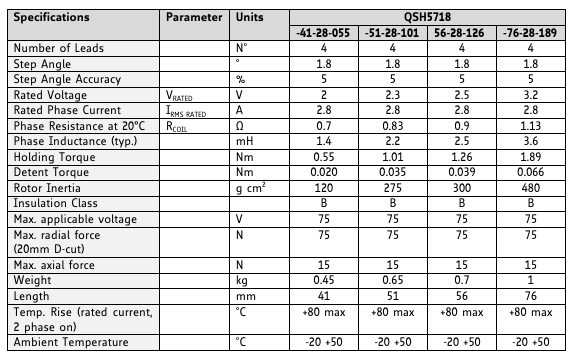
\includegraphics[scale=1]{img/qsh-serie.png}
	\caption{Specifications of QSH5718 Series}
	\label{fig:Specifications of QSH5718 Series}
\end{figure}



\includepdf[pages=6-7]{cad/QSH5718_manual.pdf}
\includepdf[pages=10]{cad/QSH5718_manual.pdf}
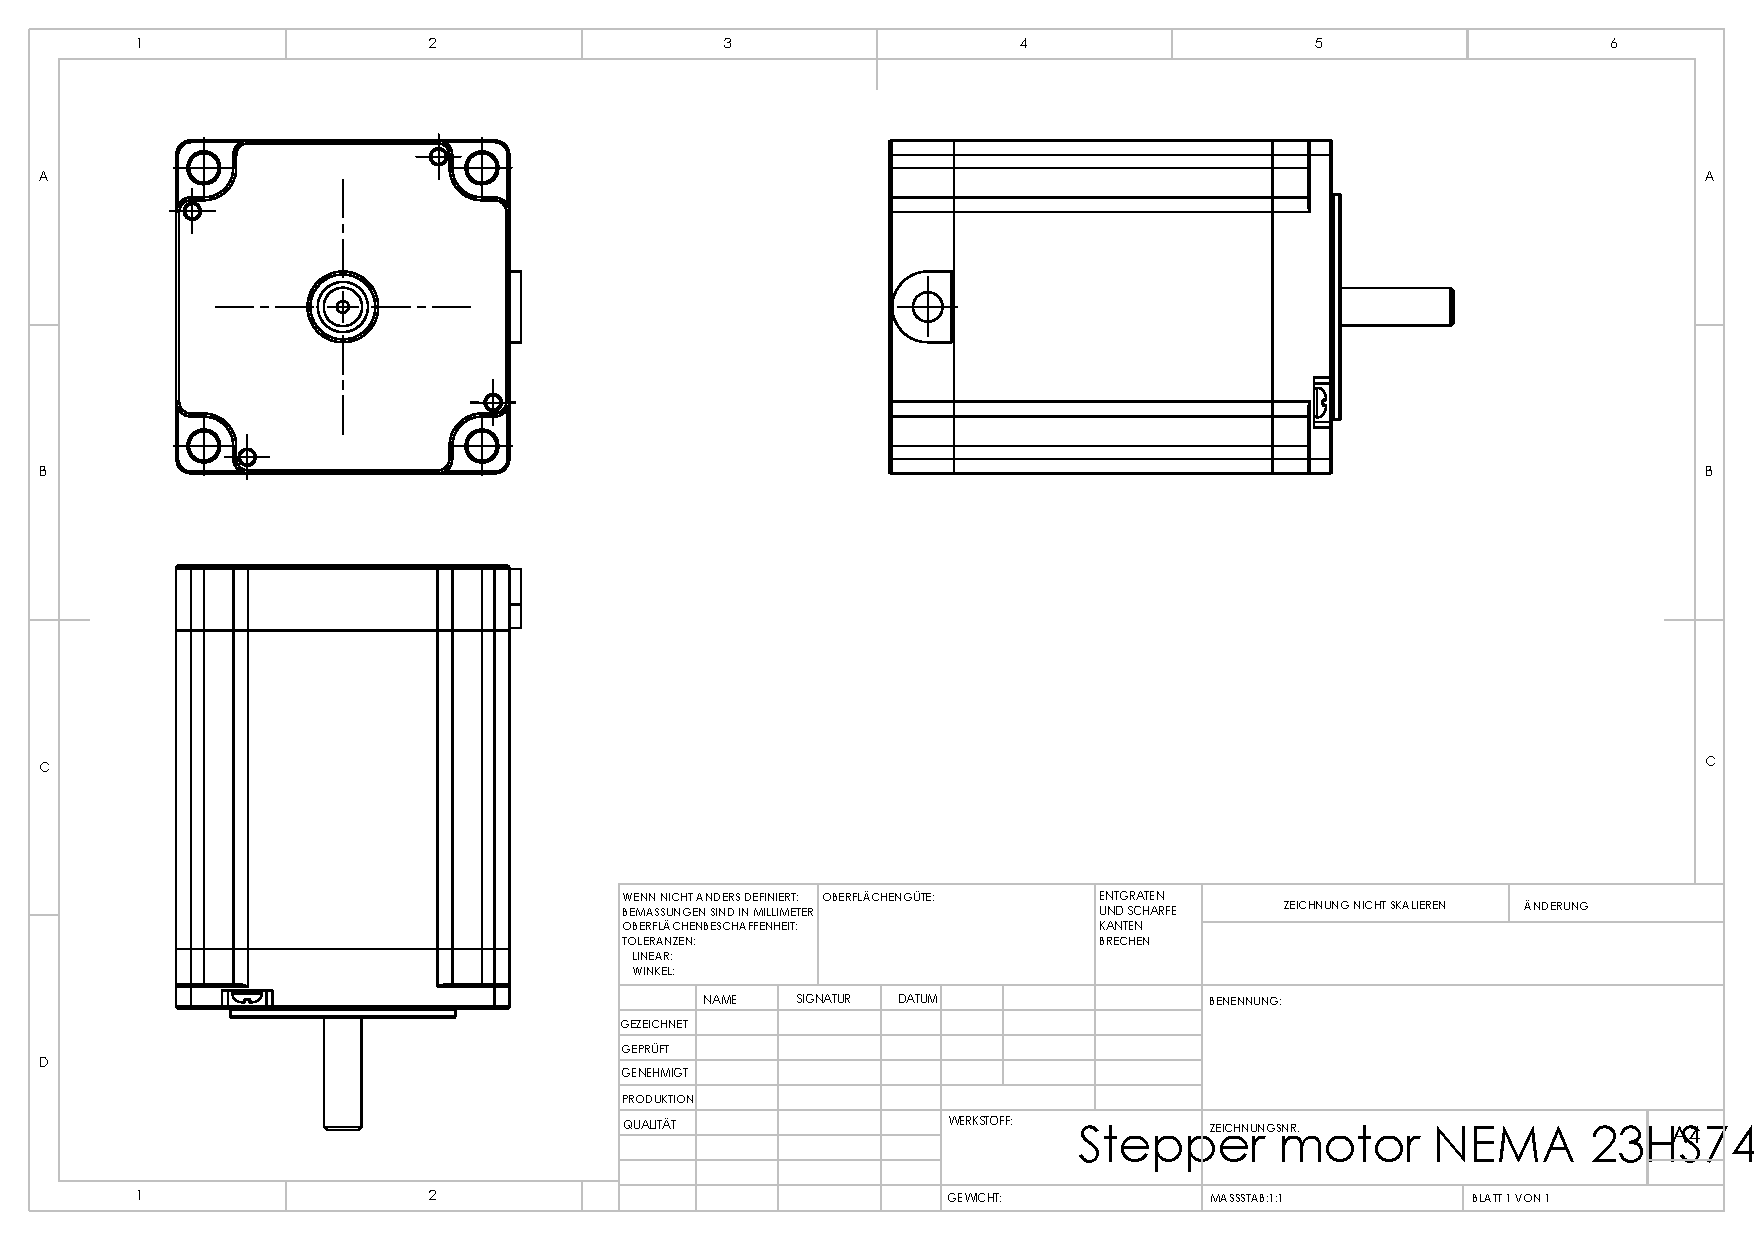
\includepdf[pages=-,landscape]{cad/Stepper-motor-NEMA-23HS7430.PDF}
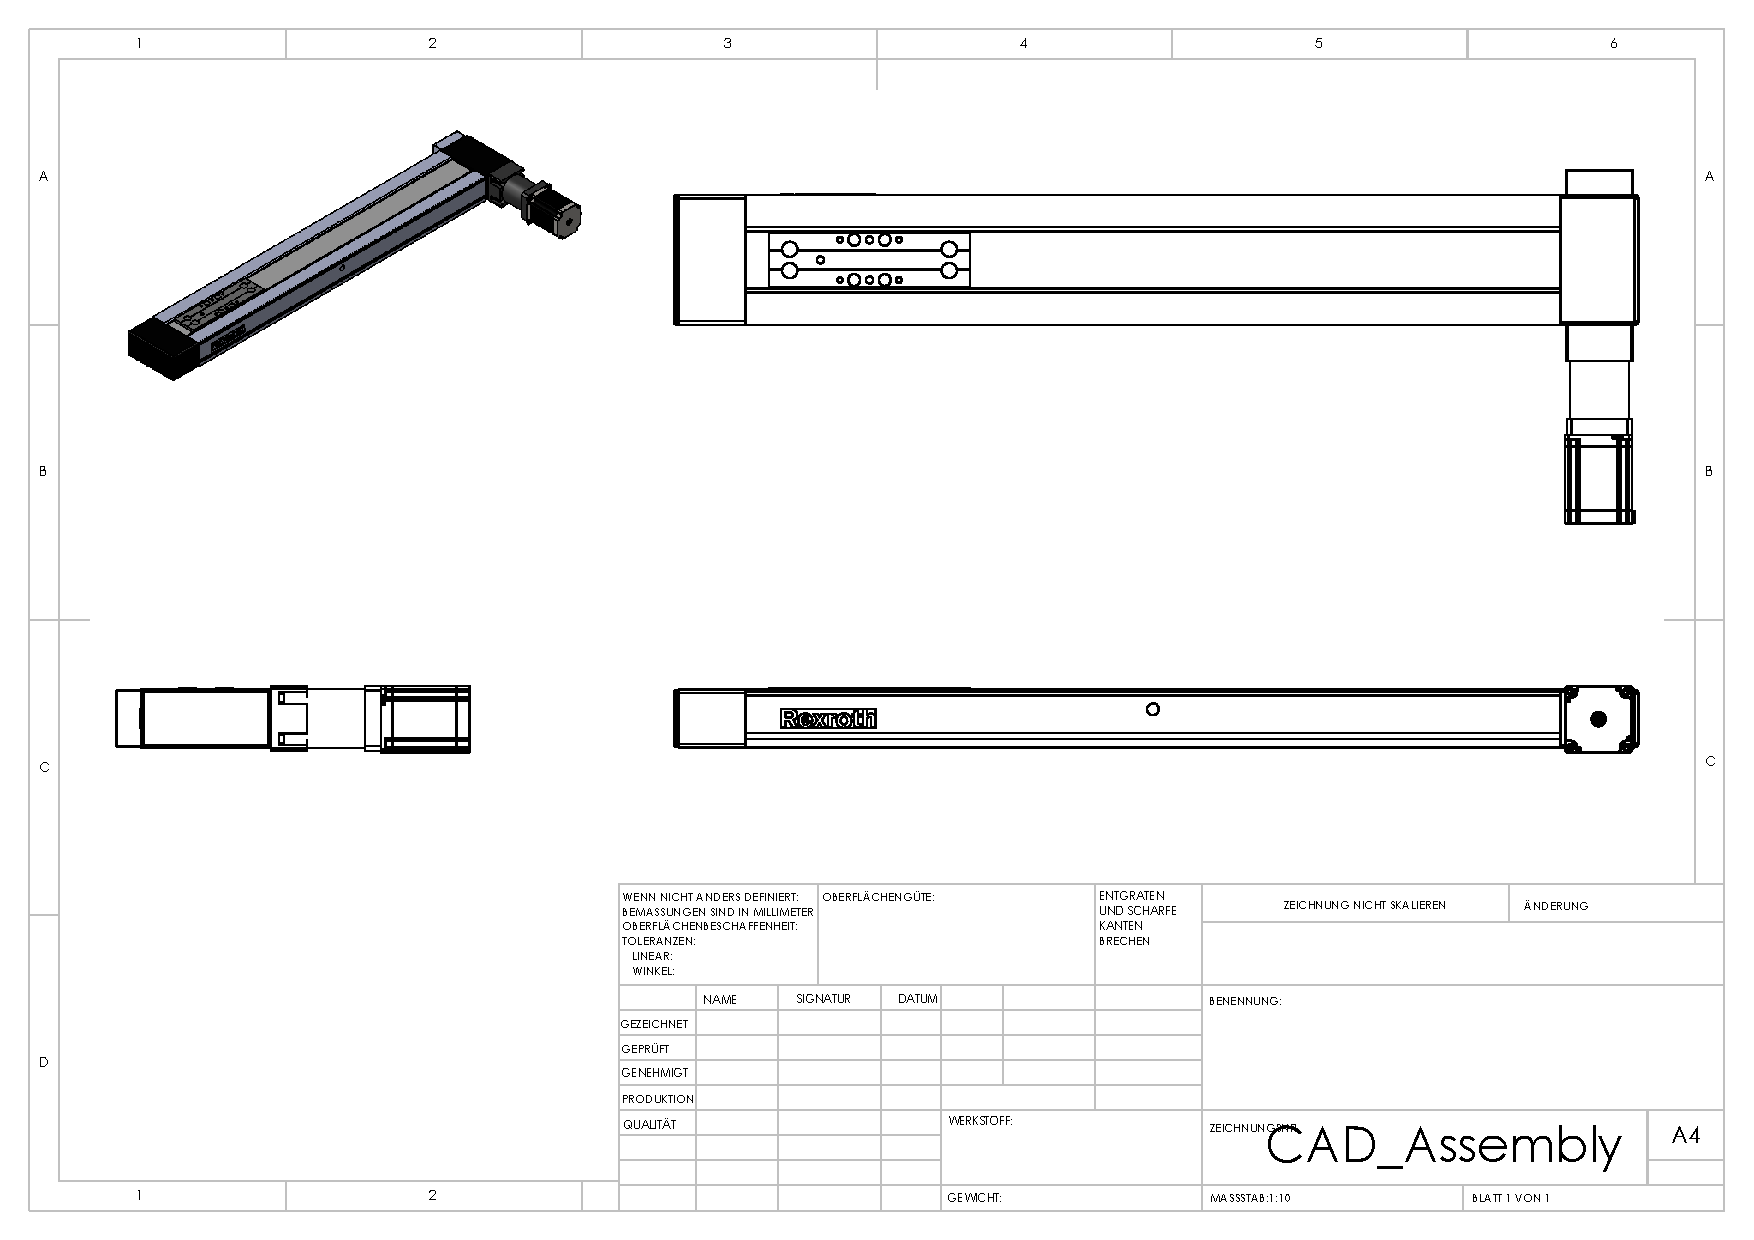
\includepdf[pages=-,landscape]{cad/CAD_Assembly.PDF}

	%###################################################
	%	Electronic
	%###################################################
\newpage
\section{Electronics}
\subsection{External motor control unit}

The external motor control unit consists of 2 different boards. One board is responsible for communication and translates the commands from the Andriox controler to the actual PWM signal and direction output. Another part of this unit is the motor controller. As the requirement, our stepper motor is bipolar and contents 4 wires. Two in a pair and each pair is only responsible for one coil.\\

\begin{figure}[h!]
	\centering
	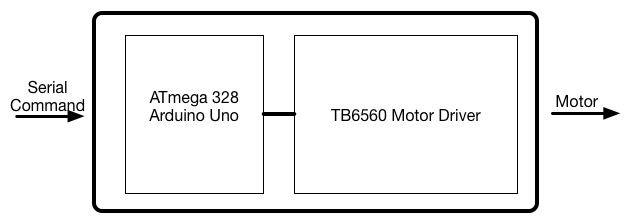
\includegraphics[scale=0.5]{img/ECU-inter.jpg}
	\caption{ECU Overview}
	\label{fig:ECU Overview}
\end{figure}

For communication we decided to use a prototype board - Arduino uno. On the board is a ATmega 328 and has built-in serial communication pins. The standard Arduino IDE has pre implemented libraries for both serial and PWM signals.\\

The same as the describtion from the NEMA 23 Motor data sheet, we also found a stepper motor driver with required output current. The core of this board is a Toshiba dual H-bridge chip TB6560.\\

%Motor Requierment and Data sheet from tb6560 motor driver
\begin{table}[h!]
\centering
\begin{tabular}{ ||l | l ||}
	\hline
	Model & QSH 5718-76-28-189\\
	Max. Voltage & 75 V\\
	Rated phase current & 2.8 A\\
	Number of leads & 4\\
	\hline
\end{tabular}
\caption{NEMA 23 requierment} 
\end{table}
\begin{table}[h!]
\centering
\begin{tabular}{|| l | l ||}
	\hline
	Operating Voltage & 12 - 36 V\\
	Max. Output current & 1.5 - 3 A/phase\\
	Drive type & Double-pole const. PWM\\
	Compatible Stepper motors & 4/6/8 leads\\
	\hline
\end{tabular}
\caption{TB6560 Data sheet} 
\end{table}

\begin{figure}[h!]
	\centering
	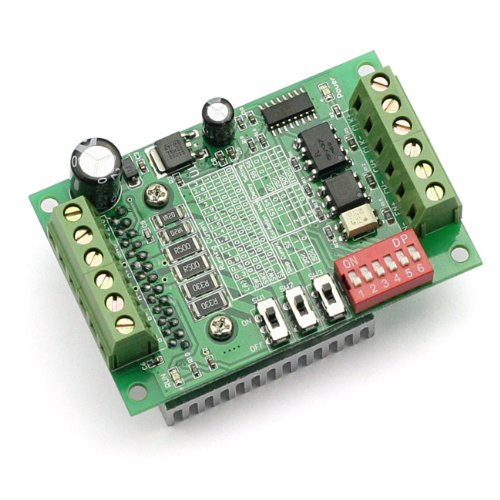
\includegraphics[scale=0.3]{img/TB6560-front.jpg}
	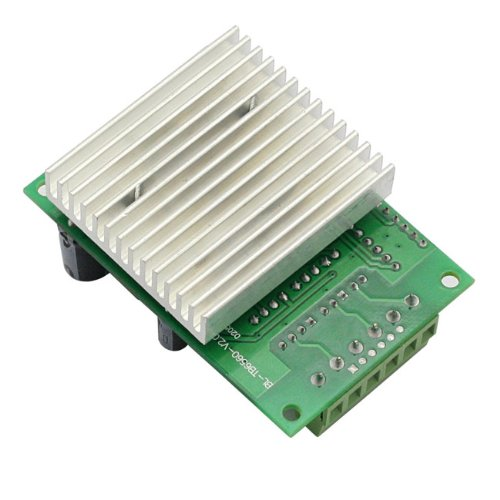
\includegraphics[scale=0.3]{img/TB6560-back.jpg}
	\caption{TB6560 Stepper Motor Driver Module}
	\label{fig:TB6560 Stepper Motor Driver Module}
\end{figure}

\subsection{Power supply}

As we are suppplying our motor with 12V, the calculation of the power consumption will be like this:\\

\begin{equation}
   \text{Total power }P_t  = \text{External Control Unit } P_e + \text{Motor }P_m
\end{equation}
\begin{equation}
   P_m = I_o \times U_i = 3A \times 12V = 36 W 
\end{equation}
\begin{equation}
   P_m \gg P_e \text{ ,so }  P_m \approx P_t
\end{equation}
\\

Our power supply must able to supply at least 40 Watts of power to drive our converying belt and control units.

\newpage
\subsection{Overall circuit}

\begin{figure}[h!]
	\centering
	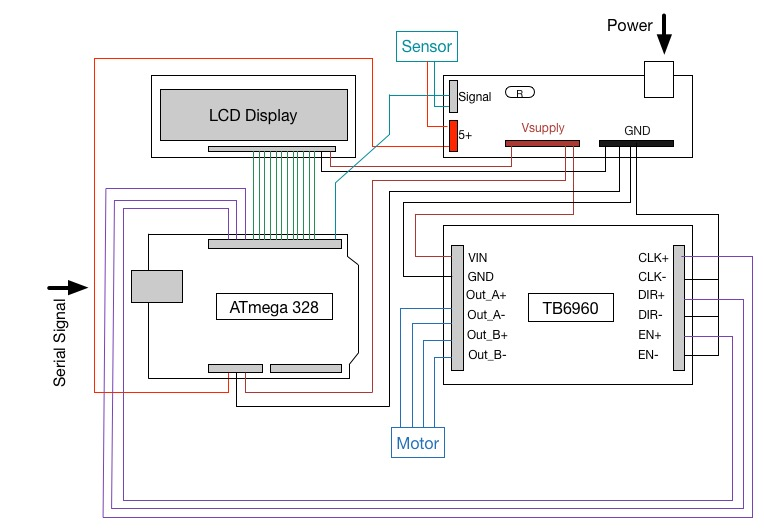
\includegraphics[scale=0.8,angle=90]{img/ECU.jpg}
	\caption{External Control Unit: cabling}
	\label{fig:External Control Unit: cabling}
\end{figure}

	%###################################################
	%	Software
	%###################################################
\newpage
\section{Software - Ecu}
\subsection{Logical equivalence }
The system logic of the external motor controller has 3 main states: initial, processing and waiting process:\\
\begin{figure}[h!]
	\centering
	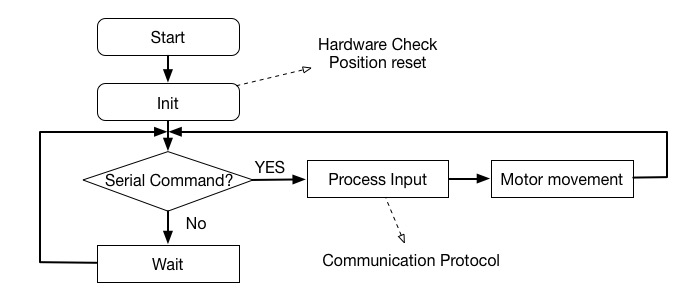
\includegraphics[scale=0.7]{img/Software-flow.jpg}
	\caption{Software Logic}
	\label{fig:Software logic}
\end{figure}\\

In the boot up phase, the system will first check if all the hardware is connected and reset the position automatically. It sends continuous signals to the motor to move the conveying base back to the origin and if the base has a physical contact with it, the digital sensor will set its output to HIGH.\\

After the reboot, the system is ready and waits for the serial command from the andrix or PCs. The serial bandwidth has already been set in the initial process and the default is 9600bit/s. Any serial signal during the waiting phase will be stored in a String buffer to futher process. The conmunication will be base on the protocol from \textbf{section 6.3}.

\subsection{Function description}
To find more detail of a specific function, please go to \textbf{section 6.4}.\\
\begin{table}[h!]
\centering
\begin{tabular}{ |l | l | c |c |}
	\hline
	Name & Use & Input & Return\\
	\hline
	setup() & Init Setup & --- & ---\\
	loop() & Main loop & --- & depend\\
	serialEvent() & Reading Serial Input and buffer them & --- & ---\\
	reset() & Reset position to origin & --- & ---\\
	goToPosition() & Go to position & Integer & ---\\
	lcdShow() & Display message on LCD Display & String 1,2 & ---\\
	lcdBackLightOnOff()   & Turn LCD Light On or Off & boolean & ---\\
	\hline
	
\end{tabular}
\end{table}

\newpage
\subsection{Communication protocol}
\begin{table}[h!]
\centering
\begin{tabular}{ ||l | l | l ||}
	\hline
	Command & Description & Sample\\
	...@ & @ - end; ... - Commands & Bandwith = 9600 bit/sec \\ \hline\hline
	ENA@ &Enable the motor & Send: \textbf{ENA@} -- Motor enabled\\
	DIS@ &Disable the motor& Send: \textbf{DIS@} -- Motor disabled\\
	RES@ &Reset, back to origin& Send: \textbf{RES@} -- Axis back to 0 position\\
	GTP...@ & Go to xxx/10 mm position	[Max. 4950]& Send: \textbf{GTP1234@} -- Axis go to 123.4mm\\
	SST...@ & Set delay of motor(default 0)	[2 byte]& Send: \textbf{SST1@} -- Set 1 ms delay for each step\\
	CTP@ & send back to the current position [2 byte]& Send: \textbf{CTP@};Return: \textbf{123@}  -- Current Position\\
	CTS@ & send back the current speed(delay) [2 byte]& Send: \textbf{CTS@};Return: \textbf{1@}  -- Current Delay\\	
	LED...@ & Turn LED Display light ON or Off & Send: \textbf{LED1@}--Light turn On\\
		\hline
\end{tabular}
\caption{Protocol: Stepper Motor Control} 
\end{table}

If you want to modify the setting of the communication bandwidth, you will have to programme the external control unit with the source code from \textbf{6.4} using Arduino IDE.\\

\textbf{Communication sample:}
\begin{lstlisting}
Normal Operation:
1.SEND:		ENA@		\\Enables the motor
2.SEND:		GTP1000@	\\Go to Position 10cm
3.SEND:		RES@		\\Reset position to 0, all default value


Move Slowly:
1.SEND:		ENA@		\\Enables the motor
2.SEND:		SST1@		\\Set Delay for 1ms
3.SEND:		GTP500@		\\Convayingbelt will move slowly to 5cm


Let conveyor belt to be able to move by hand:
1.SEND:		DIS@		\\Disable the motor
2.SEND:		RES@		\\WARNING:You must reset the position!


Turn On/Off LED Display backlight:
1.SEND:		LED1@		\\Turn On light
2.SEND:		LED0@		\\Turn Off light
3.SEND:		LED3@		\\Turn On light(Any num.>0 will be 'ON')

\end{lstlisting}


\newpage
\subsection{Source code}
\lstinputlisting[language=C]{code/Stepper_Low_Power.c}


%----------------------------------------------------------------------------------------
%	CONCLUTION
%----------------------------------------------------------------------------------------
\newpage
\part{Conclution} 
After assembling the mechanical design and putting all electronic components together, we devised a very simple system. We tested the axis accuracy and it is much more percise than we first expected.\\
\section{Resaults and Comparison}

In comparison with some of the industrial standard machines, our solution can be up to 10 times cheaper. Of course, the standard system can control/supply multiple linear or even other kinds of axises at the same time. But one of the biggest advantages of distributed system is flexibility.\\

Unter the same kind of hardware structure, we are able to connect multiple controllers with a central computer, and control them induvidually. It is also even posible to implement some kind of smart algorithm, which is designed spicificly for each individual enviroment.\\

In this example we only show one way of using an Andrix controller in Industrial area. It shows us the potential of distributed system and can be one of the most important keys for 'Industrial 4.0'. It will change the way we look at the normal rigid structure.\\


\end{document}
\grid
\grid
